%%%%%%%%%%%%%%%%%%%%%%%%%%%%%%%%%%%%%%%%%
% Short Sectioned Assignment
% LaTeX Template
% Version 1.0 (5/5/12)
%
% This template has been downloaded from:
% http://www.LaTeXTemplates.com
%
% Original author:
% Frits Wenneker (http://www.howtotex.com)
%
% License:
% CC BY-NC-SA 3.0 (http://creativecommons.org/licenses/by-nc-sa/3.0/)
%
%%%%%%%%%%%%%%%%%%%%%%%%%%%%%%%%%%%%%%%%%

%----------------------------------------------------------------------------------------
%	PACKAGES AND OTHER DOCUMENT CONFIGURATIONS
%----------------------------------------------------------------------------------------

\documentclass[paper=a4, fontsize=11pt]{scrartcl} % A4 paper and 10pt font size

\usepackage[T1]{fontenc} % Use 8-bit encoding that has 256 glyphs
%\usepackage{fourier} % Use the Adobe Utopia font for the document - comment this line to return to the LaTeX default
\usepackage[english]{babel} % English language/hyphenation
\usepackage{amsmath,amsfonts,amsthm} % Math packages
\usepackage{graphicx}
\usepackage{lipsum} % Used for inserting dummy 'Lorem ipsum' text into the template
\usepackage{float}
\usepackage{sectsty} % Allows customizing section commands
\allsectionsfont{\normalfont\scshape} % Make all sections centered, the default font and small caps
\usepackage{url}

\usepackage{fancyhdr} % Custom headers and footers


\usepackage{listings}
\usepackage{xcolor}
\usepackage[section]{placeins}
\colorlet{punct}{red!60!black}
\definecolor{background}{HTML}{EEEEEE}
\definecolor{delim}{RGB}{20,105,176}
\colorlet{numb}{magenta!60!black}

\lstdefinelanguage{json}{
    basicstyle=\normalfont\ttfamily,
    numbers=left,
    numberstyle=\scriptsize,
    stepnumber=1,
    numbersep=8pt,
    showstringspaces=false,
    breaklines=true,
    frame=lines,
    backgroundcolor=\color{background},
    literate=
     *{0}{{{\color{numb}0}}}{1}
      {1}{{{\color{numb}1}}}{1}
      {2}{{{\color{numb}2}}}{1}
      {3}{{{\color{numb}3}}}{1}
      {4}{{{\color{numb}4}}}{1}
      {5}{{{\color{numb}5}}}{1}
      {6}{{{\color{numb}6}}}{1}
      {7}{{{\color{numb}7}}}{1}
      {8}{{{\color{numb}8}}}{1}
      {9}{{{\color{numb}9}}}{1}
      {:}{{{\color{punct}{:}}}}{1}
      {,}{{{\color{punct}{,}}}}{1}
      {\{}{{{\color{delim}{\{}}}}{1}
      {\}}{{{\color{delim}{\}}}}}{1}
      {[}{{{\color{delim}{[}}}}{1}
      {]}{{{\color{delim}{]}}}}{1},
}


\lstdefinelanguage{python}{
    basicstyle=\normalfont\ttfamily,
    numbers=left,
    numberstyle=\scriptsize,
    stepnumber=1,
    numbersep=8pt,
    showstringspaces=false,
    breaklines=true,
    frame=lines,
    backgroundcolor=\color{background},
    literate=
     *{0}{{{\color{numb}0}}}{1}
      {1}{{{\color{numb}1}}}{1}
      {2}{{{\color{numb}2}}}{1}
      {3}{{{\color{numb}3}}}{1}
      {4}{{{\color{numb}4}}}{1}
      {5}{{{\color{numb}5}}}{1}
      {6}{{{\color{numb}6}}}{1}
      {7}{{{\color{numb}7}}}{1}
      {8}{{{\color{numb}8}}}{1}
      {9}{{{\color{numb}9}}}{1}
      {:}{{{\color{punct}{:}}}}{1}
      {,}{{{\color{punct}{,}}}}{1}
      {\{}{{{\color{delim}{\{}}}}{1}
      {\}}{{{\color{delim}{\}}}}}{1}
      {[}{{{\color{delim}{[}}}}{1}
      {]}{{{\color{delim}{]}}}}{1},
}



\pagestyle{fancyplain} % Makes all pages in the document conform to the custom headers and footers
\fancyhead{} % No page header - if you want one, create it in the same way as the footers below
\fancyfoot[L]{} % Empty left footer
\fancyfoot[C]{} % Empty center footer
\fancyfoot[R]{\thepage} % Page numbering for right footer
\renewcommand{\headrulewidth}{0pt} % Remove header underlines
\renewcommand{\footrulewidth}{0pt} % Remove footer underlines
\setlength{\headheight}{13.6pt} % Customize the height of the header
\usepackage{authblk}
\usepackage[margin=0.89in]{geometry}
\numberwithin{equation}{section} % Number equations within sections (i.e. 1.1, 1.2, 2.1, 2.2 instead of 1, 2, 3, 4)
\numberwithin{figure}{section} % Number figures within sections (i.e. 1.1, 1.2, 2.1, 2.2 instead of 1, 2, 3, 4)
\numberwithin{table}{section} % Number tables within sections (i.e. 1.1, 1.2, 2.1, 2.2 instead of 1, 2, 3, 4)

\setlength\parindent{0pt} % Removes all indentation from paragraphs - comment this line for an assignment with lots of text

%----------------------------------------------------------------------------------------
%	TITLE SECTION
%----------------------------------------------------------------------------------------

\newcommand{\horrule}[1]{\rule{\linewidth}{#1}} % Create horizontal rule command with 1 argument of height

\title{	
\normalfont \normalsize 
\textsc{The Ohio State University, Department of Computer Science and Engineering} \\ [25pt] % Your university, school and/or department name(s)
\horrule{0.5pt} \\[0.4cm] % Thin top horizontal rule
\huge Homework 6: Prediction of rating from Yelp review text % The assignment title
\horrule{2pt} \\[0.5cm] % Thick bottom horizontal rule
}

\author{Grover, Karan \& Arora, Pragya \& Ghai, Piyush}
\affil{\textit {\{grover.120, arora.170, ghai.8\}@osu.edu}}

\date{\normalsize\today} % Today's date or a custom date

\begin{document}
\maketitle % Print the title
\newpage
%----------------------------------------------------------------------------------------
%	PROBLEM 1
%----------------------------------------------------------------------------------------
\section{Problem Statement}
\subsection{About Yelp}
\textbf{Yelp} \cite{yelp} a famous website as well as a mobile app which publishes crowd sourced reviews about food joints and businesses. It also has a division which handles online reservations for restaurants. \textbf{Yelp Dataset Challenge}\cite{yelp_dataset_challenge} is a publicly open contest sponsored by Yelp, in which the participants are challenged to use Yelp's data in an innovative way. \\
\subsection{Our Mission}
The Yelp dataset downloaded from Yelp dataset challenge website is huge and consists of over 9M reviews by roughly 687k users for over 86k businesses \cite{yelp_dataset_challenge}. For this project, we chose to predict a review's rating based on the review text. The rating will be done on a scale of 1-5, where 1 stands for awful and 5 stands for excellent. We built multiple models and accessed which models would fit our use case the best. This is explained in more depth in the later sections of this report.

\subsection{About the dataset}
The Yelp Dataset consists of several files in JSON format of the data. The main files as per our use-case were the \textit{yelp\_academic\_dataset\_business.json} \& \textit{yelp\_academic\_dataset\_review.json}. The two data files were \textbf{2.13 GB} \& \textbf{73.6MB} in size respectively. The data representation in the for acadmic\_dataset\_business is as follows : \\
\begin{lstlisting}[language=json]
{
    "type": "business",
    "business_id": (encrypted business id),
    "name": (business name),
    "neighborhoods": [(hood names)],
    "full_address": (localized address),
    "city": (city),
    "state": (state),
    "latitude": latitude,
    "longitude": longitude,
    "stars": (star rating, rounded to half-stars),
    "review_count": review count,
    "categories": [(localized category names)]
    "open": True / False (corresponds to closed, not business hours),
    "hours": {
        (day_of_week): {
            "open": (HH:MM),
            "close": (HH:MM)
        },
        ...
    },
    "attributes": {
        (attribute_name): (attribute_value),
    },
}
\end{lstlisting}
The data representation in the for acadmic\_dataset\_review is as follows : \\
\begin{lstlisting}[language=json]
{   "type": "review",
    "business_id": (encrypted business id),
    "user_id": (encrypted user id),
    "stars": (star rating, rounded to half-stars),
    "text": (review text),
    "date": (date, formatted like "2012-03-14"),
    "votes": {(vote type): (count)},
}
\end{lstlisting}
The given datasets were first converted and exported into csv formats using a simple python script. The python script is a part of the \textbf{PreProcessing1.py} python file.

%% TODO Insert more sections here
\section{Exploratory Analysis of Yelp Dataset}
The primary features of interest to us in the given dataset are \textbf{reviews} by the user, the \textbf{stars} associated with a review and the business establishment the reviews belong to. After merging the business dataset and the review dataset, we analysed which business unit the maximum reviews belonged to. Table \ref{review_cat_table} lists out randomly sampled 10 rows from the dataset. In figure \ref{category_reviews}, the x-axis was chosen as numeric in order to display a cleaner graph, but the sharp spike corresponds to \textit{restaurant} as the main category. The total review count is close to 1.6M for this category.
Next we thought of finding the geographical split of the reviews. The Yelp dataset consists of data collected from \textit{29} different states. Table \ref{state_review} shows the split of review count over all business establishments sorted by the top 7 states. 
As we can see, the maximum reviews come from Nevada, followed by Arizona, both of which are over 1M in number. After Arizona, the next highest is North Carolina, which is nearly one-tenth lesser than that of Arizona. This could perhaps be indicative of a very strong presence of Yelp in business establishments in NV and AZ as opposed to other states.\\

Since there are so many reviews for restaurant, we decided to focus on the subset of reviews for restaurants ( the subset is obtained in the pre-processing step) for further analysis.  
Next we observed the variation of average rating stars against the \textit{length of the reviews (in characters)}. The average rating varies quite a lot for reviews with higher number of characters, indicating that the polarity of reviews fluctuates a lot more from one length to another. There is less fluctation in the average rating of reviews from length ~50 to ~500 characters. Hence we chose to subset the reviews based on minimum and maximum length threshholds. Figure \ref{average_length} indicates this observed trend. Another motive for reducing the subset for reviews is based from inferences drawn from Figure \ref{length_count}. From this we can see that the total number of length >700 is very less as compared to the overall size of the review corpus. Thus combining the analysis from this and the previous figure, we subsetted the number of reviews.\\

Next we observed the distribution of reviews with the star rating, i.e. what review was given which star by a user. From Figure \ref{star_distribution}, we can see that there is a skewed distribution of reviews in terms of star ratings they have received. A majority of reviews have a 5 star or a 4 star rating, while the count for 1 star is the lowest. This will later on form a basis for us to create training datasets based on data sampled from each star rating, in order to ensure even representation in the training corpus.

\subsection{Word Cloud}
Given the distribution of reviews, we decided to capture the common sentiment for all the reviews individually. We did this by plotting a wordcloud of review texts grouped by their star rating. To do this, we preprocessed the review texts to remove all the common stop  words, tokenized the words and then plotted them. Figures \ref{wc1}, \ref{wc2}, \ref{wc3}, \ref{wc4}, \ref{wc5} represent this pictorially.

\begin{table}[!htb]
 \centering
 \caption{Categories and sub categories a review belongs to in the Yelp business dataset}
 \label{review_cat_table}
 \begin{tabular}{l l} 
    \noalign{\smallskip}\hline\noalign{\smallskip}
    ReviewId & Categories \\
    \noalign{\smallskip}\hline\noalign{\smallskip}
	QPTBica7UkkrT7xEQskBww & [Nightlife, Bars, American (Traditional)] \\
O93XUShpjG7X\_VioaN0ViQ & [Local Services, Mobile Phone Repair] \\
5zvonAPvVG17Aid1MZYFGw & [Food, Coffee \& Tea] \\
UrA\_eN4seEdDLZR-gIrG4g & [Skin Care, Weight Loss Centers] \\
vZSNSfzb7XDMpBXr\_PEX1w & [Music Venues, Arts \& Entertainment] \\
CEO6MmROql9ZFHKTQ1FXow  & [Bars, American (Traditional), Food] \\
lH-jQdLKKGcG-3DzgMgLQA & [Thai, Restaurants] \\
ctbEMtUouLPzf2F25DQamw & [Tires, Automotive] \\
iESG5qEoUNYJ4lOOv0337g & [Burgers, American (New), Restaurants] \\
w0LtO11Ylu-7wnzKs1E9QA & [Sushi Bars, Asian Fusion, Restaurants] \\
    \noalign{\smallskip}\hline
  \end{tabular} 
\end{table}  

\begin{figure}[!htb]
\centering
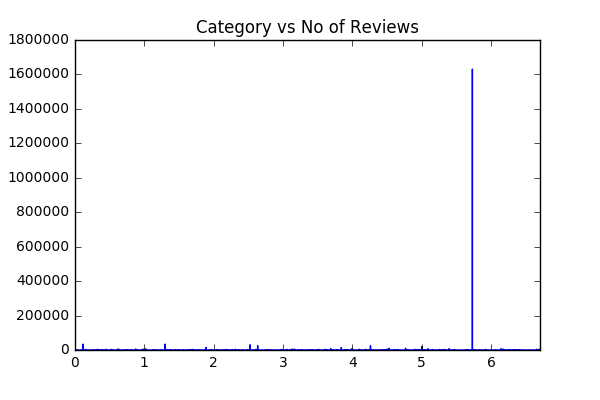
\includegraphics[width=300px, height = 250px]{category_reviews.png}
\caption{Review count v/s category they belong to}
\label{category_reviews}
\end{figure} 

\begin{table}[!htb]
 \centering
 \caption{Review counts for different states}
 \label{state_review}
 \begin{tabular}{l l} 
    \noalign{\smallskip}\hline\noalign{\smallskip}
    State & Total Reviews \\
    \noalign{\smallskip}\hline\noalign{\smallskip}
NV & 1154799 \\
AZ & 1029103 \\
NC & 165625 \\
PA & 111542 \\
QC & 88046 \\
WI & 69917 \\
EDH & 30003 \\
    \noalign{\smallskip}\hline
  \end{tabular} 
\end{table}  

\begin{figure}[!htb]
\centering
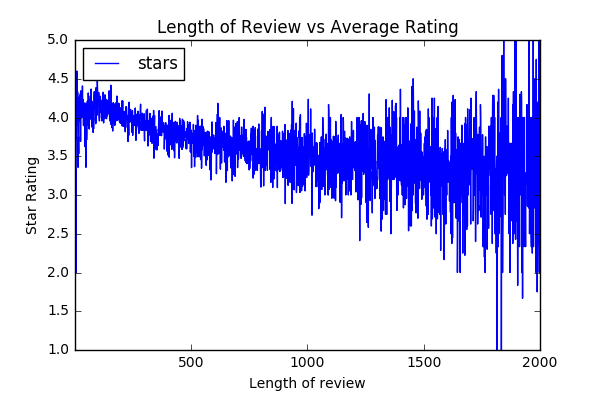
\includegraphics[width=250px, height = 200px]{avg_count.png}
\caption{Review count v/s category they belong to}
\label{average_length}
\end{figure} 

\begin{figure}[!htb]
\centering
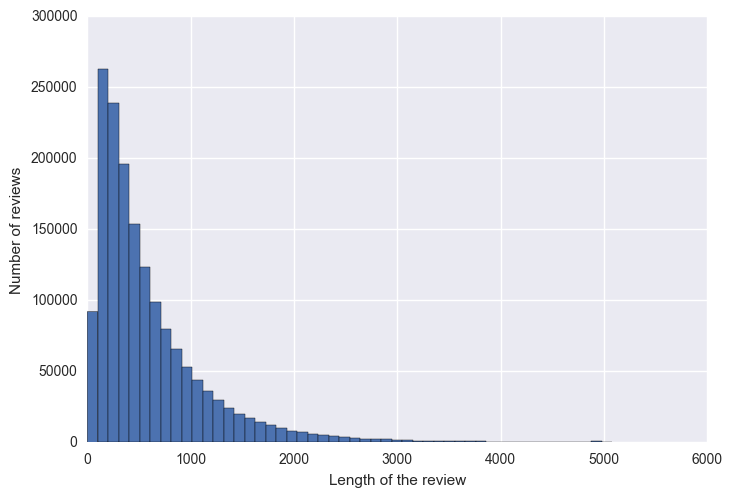
\includegraphics[width=250px, height = 200px]{len_count.png}
\caption{Length of a review v/s count of reviews}
\label{length_count}
\end{figure} 

\begin{figure}[!htb]
\centering
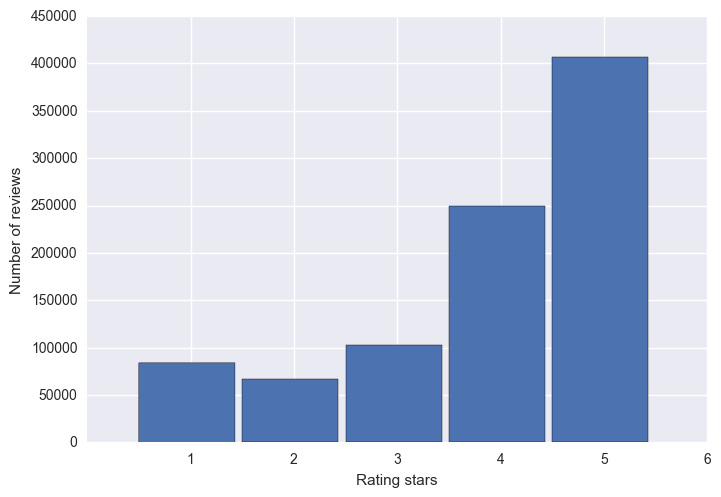
\includegraphics[width=250px, height = 200px]{star_review_count.png}
\caption{Total reviews for a given star rating}
\label{star_distribution}
\end{figure} 

\begin{figure}[!htb]
\centering
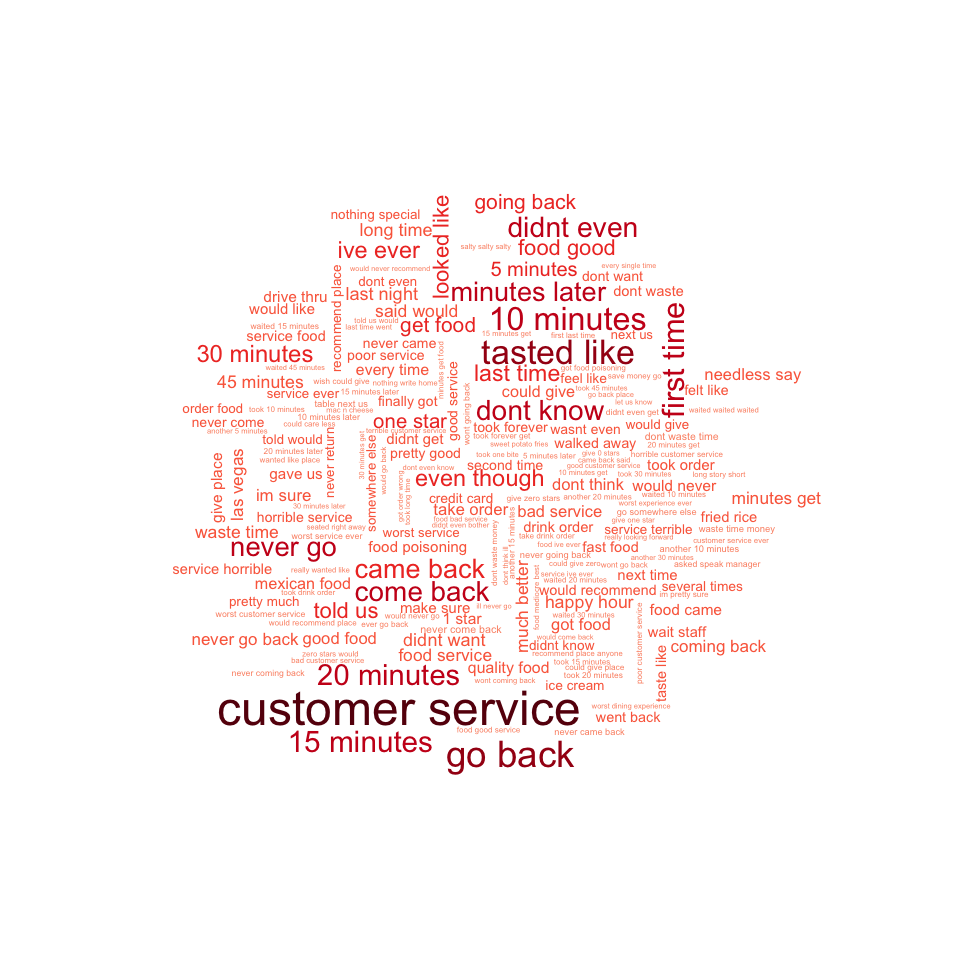
\includegraphics[width=250px, height = 200px]{1_star_wordcloud_500k.png}
\caption{Word Cloud for 1 star rating reviews}
\label{wc1}
\end{figure} 

\begin{figure}[!htb]
\centering
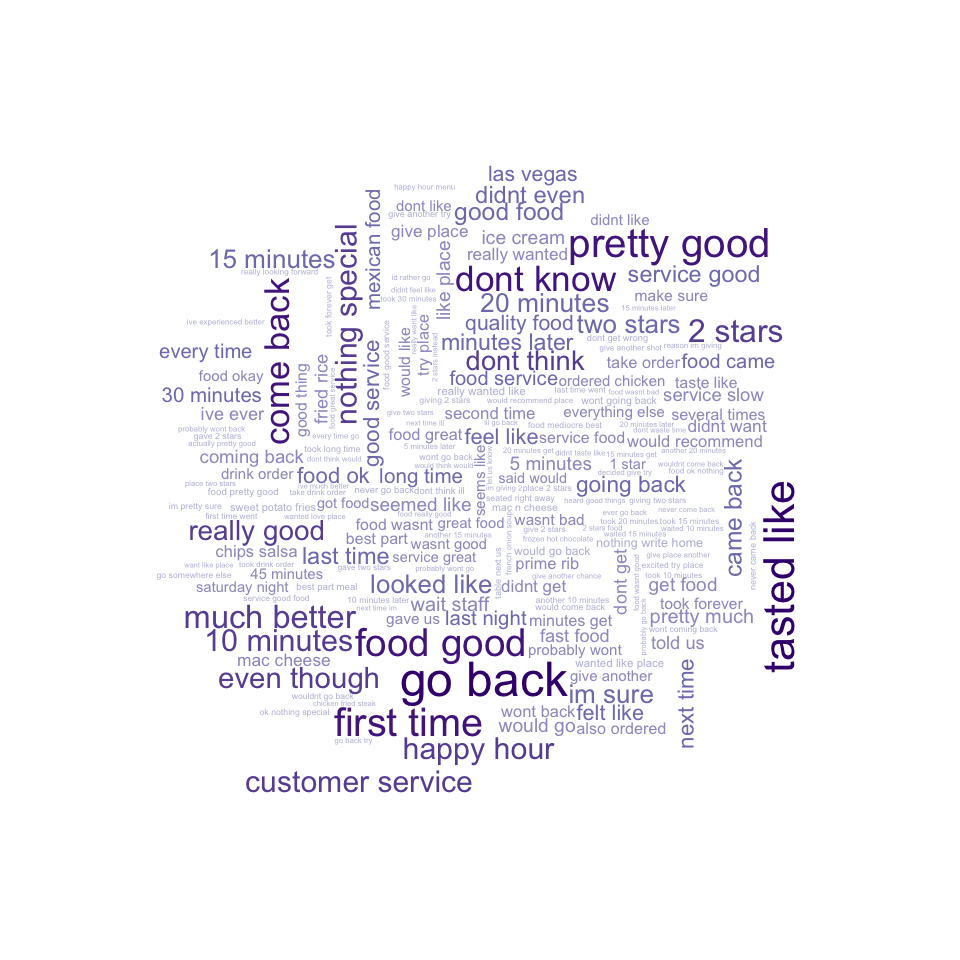
\includegraphics[width=250px, height = 200px]{2_star_wordcloud_500k.png}
\caption{Word Cloud for 2 star rating reviews}
\label{wc2}
\end{figure} 

\begin{figure}[!htb]
\centering
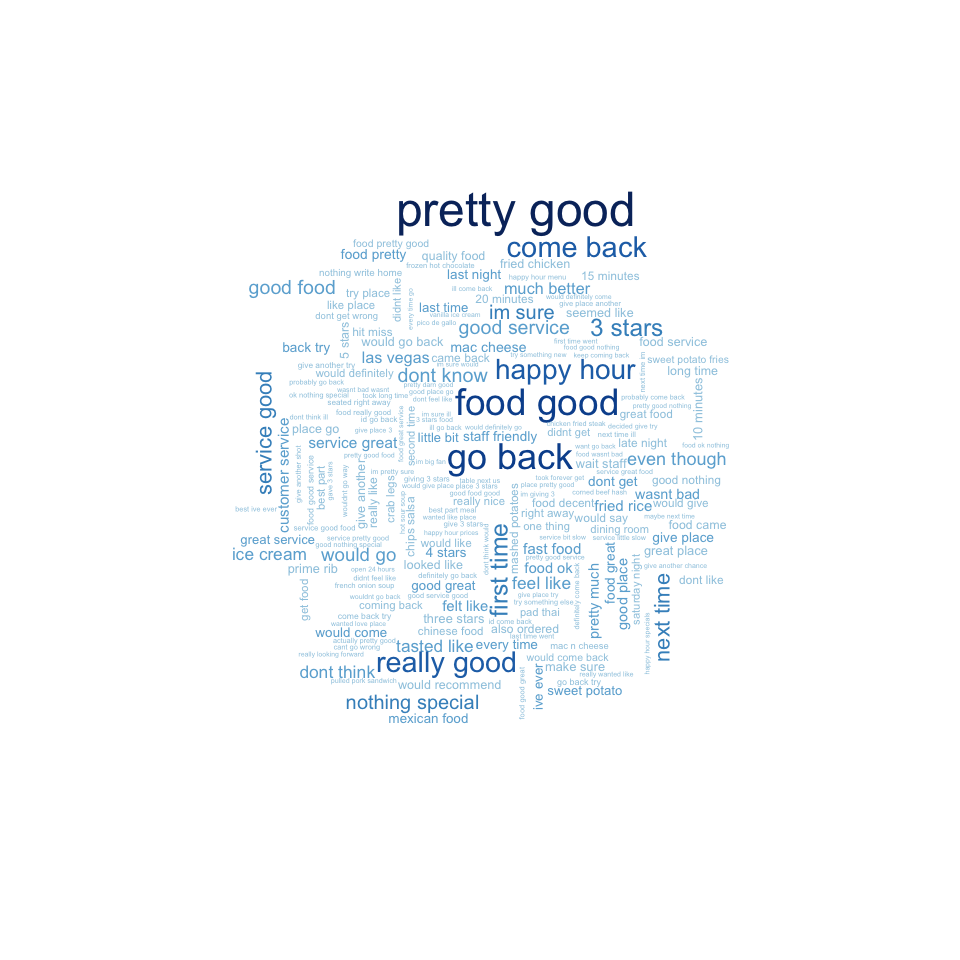
\includegraphics[width=250px, height = 200px]{3_star_wordcloud_500k.png}
\caption{Word Cloud for 3 star rating reviews}
\label{wc3}
\end{figure} 

\begin{figure}[!htb]
\centering
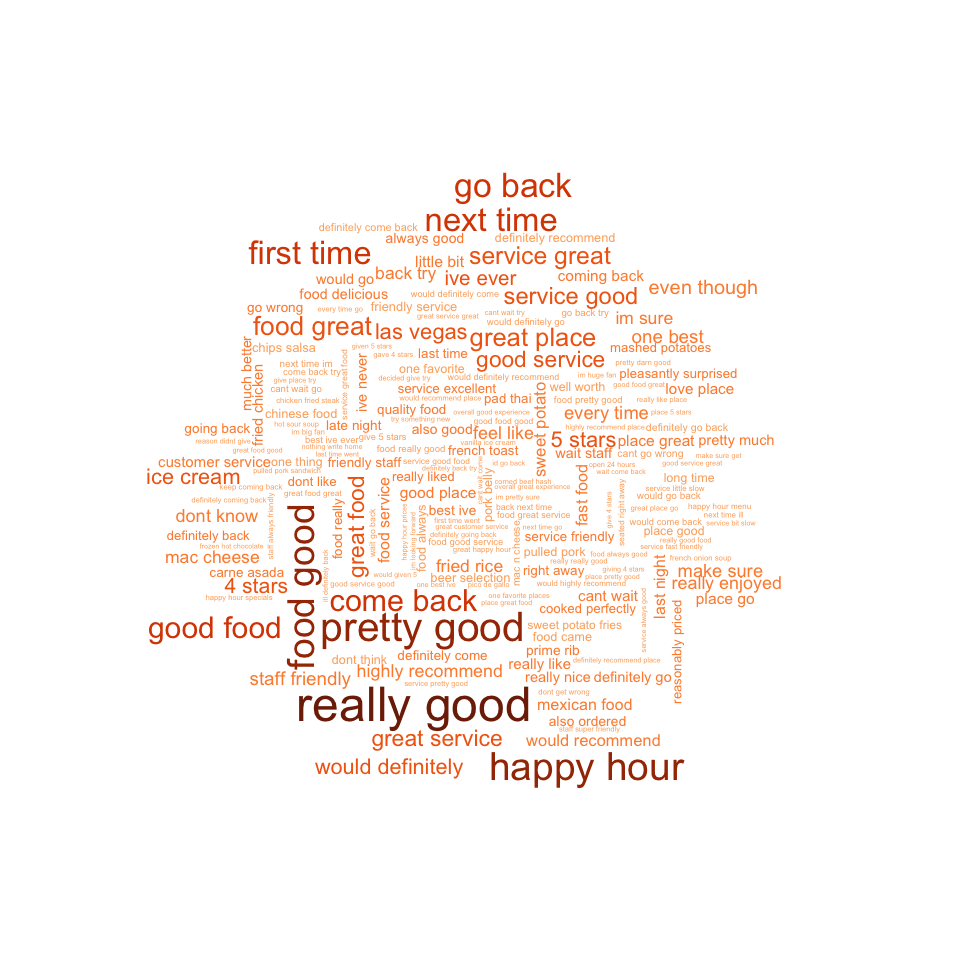
\includegraphics[width=250px, height = 200px]{4_star_wordcloud_500k.png}
\caption{Word Cloud for 4 star rating reviews}
\label{wc4}
\end{figure} 

\begin{figure}[!htb]
\centering
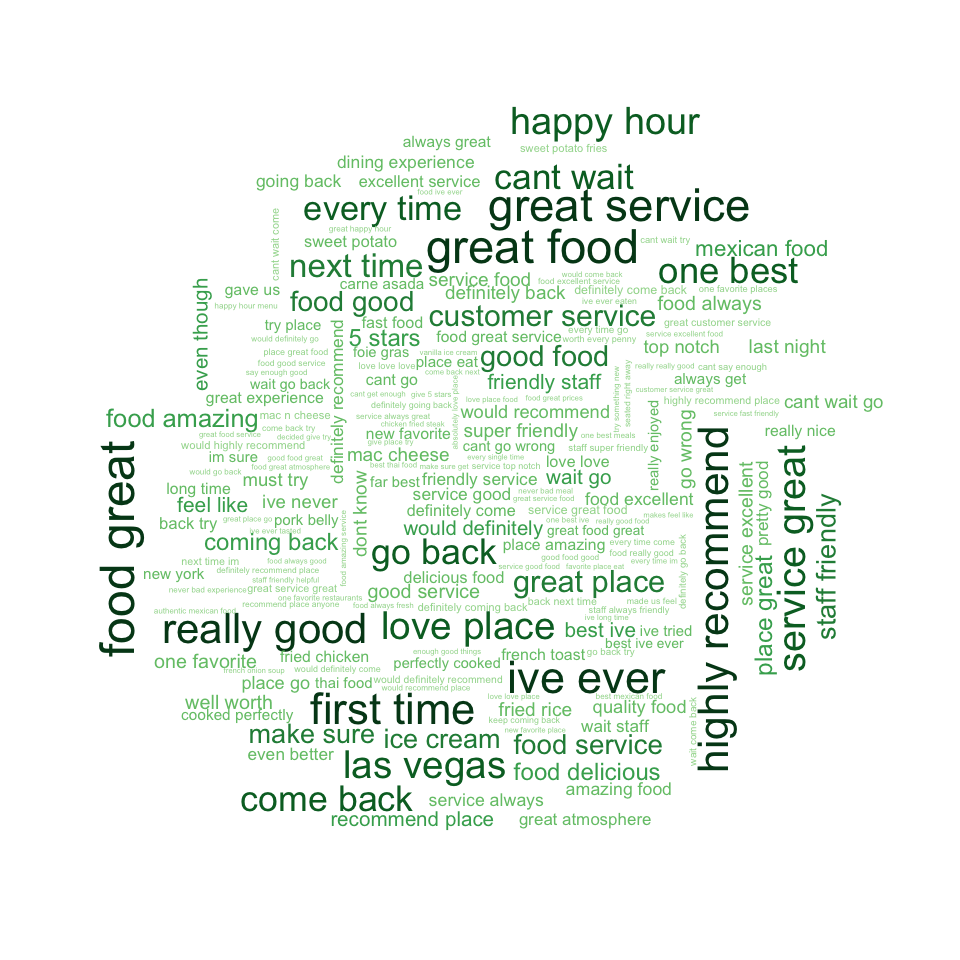
\includegraphics[width=250px, height = 200px]{5_star_wordcloud_500k.png}
\caption{Word Cloud for 5 star rating reviews}
\label{wc5}
\end{figure} 


\section{Program Description}
The code has been broken down into the following parts : 

\begin{enumerate}
\item \textbf{Pre-Processing 1}\\
In pre-processing 1, Yelp provided JSON files were converted into the CSV format. The required CSV files were loaded as Python data-frames and then merged, filtered and stored locally for later usage.

\item \textbf{Pre-Processing 2}\\
In pre-processing 2, the review text is cleaned up, grouped and stored according to the rating of the reviews, which further gets partitioned into training and testing dataset.

\item	\textbf{Models}\\
We implemented a total of 8 models and each model has been separated into a different python file. Following are the models which were implemented and compared:
\begin{itemize}
\item \textbf{Baseline model}
\item \textbf{TFIDF model}
\item \textbf{Bag of words model}
\item \textbf{Bigram model}
\item \textbf{Trigram model}
\item \textbf{Bi and Tri-gram model}
\item \textbf{LDA Model}
\item \textbf{LDA + Sentiment layer model}
\end{itemize}
\end{enumerate}

\section{Model Description}
We built several models which generated different forms of features of review text to help predict the sentiment:

\begin{figure}
\centering
\includegraphics[width=400px, height = 300px]{Models.png}
\caption{Flow chart showing the models in the workflow}
\label{models_diag}
\end{figure} 

\begin{enumerate}

\item \textbf{Baseline model}\\
In the baseline model, the average rating across all reviews is assigned as the predicted rating for each review. The average rating of all reviews was found to be 3.9 which was rounded off to 4 and used as baseline prediction. This was used as a simple benchmark for all the other models we applied to this dataset.

\item \textbf{TFIDF model}\\
In TFIDF or term frequency-inverse document frequency, each review text is represented as a vector having dimension equal to the number of words in the dictionary and each dimension representing a weight of importance of the word in the review text. This TFIDF vector representations of the review corpus become the features to the classification model.

\item \textbf{Bag of words model}\\
In the bag of words or the unigram model, the review texts are converted to term frequency vectors, where each dimension represents the count of the term in the review text. The term frequency representations of the entire corpus become the features to the classification model.

\item \textbf{Bigram model}\\
In the Bigram model, the review text is broken down into bigrams - set of two words occurring consecutively in the text and the document is then represented as the term frequency vector of these bigrams. Each dimension of the term frequency vector represents the count of the bigram in the review text. 

\item \textbf{Trigam model}\\
In the Trigram model, the review text is broken down into trigrams - set of three words occurring consecutively. The term frequency vectors of these sets become the features of the review text where each dimension represents the count of the trigram in the review text.

\item Bi and Tri-gram model\\
In the Bi and Tri-gram mode, the review text is broken down into both bi and tri-grams. The term frequency vectors of these sets become the features of a review text where each dimension represents the count of the bigram or trigram in the review text.

\item \textbf{LDA model}\\
All the previous models consider all the words/bigrams/trigrams and their frequency as the training features. In the case where the corpus is huge, the dimensionality of the input features would be huge. To reduce the dimensions, we have used the Latent Dirichlet allocation (LDA) algorithm which discovers a given number of topics or themes in the corpus. Each review text is then represented as vector of probability distribution across these topics. These topic distribution vectors become the features to the classification model.
We have used the genism package in python to create the LDA model:
\begin{lstlisting}[language=python]
{
	ldamodel = gensim.models.ldamodel.LdaModel(corpus, num_topics=15, id2word = dictionary)
}
\end{lstlisting}

Parameters:
\begin{itemize}
\item num\_topics:  The number of topics that should be discovered.
\item id2word: The dictionary created from the corpus
\end{itemize}

\item \textbf{LDA model + Sentiment Layer}
In this model, sentiment of the review was fed in as the feature alongside the topic distribution of the review. The sentiment of the review was extracted using the Naïve Bayes classifier. 
\end{enumerate}

\section{Model Evaluation}
\begin{table}[!htb]
 \centering
 \caption{Baseline model performance metrics}
 \label{baseline_performance}
 \begin{tabular}{l l l} 
    \noalign{\smallskip}\hline\noalign{\smallskip}
    Accuracy & 0.273578\\
    F1 score & 0.117535\\
    Precision & 0.074845\\
    Recall &0.273578\\
    \noalign{\smallskip}\hline
  \end{tabular} 
\end{table}  

We can see in the above table that the Baseline model, which predicts every review's rating to be the average rating of all reviews, performs poorly in terms of accuracy. Even the precision of the model is only 7.5\%.

\begin{table}[!htb]
 \centering
 \caption{TFIDF model performance metrics}
 \label{tfidf_performance}
 \begin{tabular}{l l l} 
    \noalign{\smallskip}\hline\noalign{\smallskip}
    Metric & Logistic Regression & Multinomial Naive Bayes\\
    \noalign{\smallskip}\hline\noalign{\smallskip}
    Accuracy & 0.640334	& 0.553686\\
    F1 score & 0.640334	& 0.553686\\
    Precision & 0.618353 & 0.507628\\
    recall & 0.640334 & 0.553686\\
    \noalign{\smallskip}\hline
  \end{tabular} 
\end{table}  

In the TF-IDF model, we tried two classification models - Logistic Regresion and Multinomial Naive Bayes. From the above results, we can see that Logistic Regression outperforms Multinomial Naive Bayes in terms of all metrics. The best accuracy obtained using this model is 64\%.	

\begin{table}[!htb]
 \centering
 \caption{Bag of words model performance metrics}
 \label{bow_performance}
 \begin{tabular}{l l l} 
    \noalign{\smallskip}\hline\noalign{\smallskip}
    Accuracy & 0.630097\\
    F1 score & 0.624512\\
    Precision & 0.621452\\
    recall & 0.630097\\
    \noalign{\smallskip}\hline
  \end{tabular} 
\end{table}  

\begin{table}[!htb]
 \centering
 \caption{Bigram model performance metrics}
 \label{bigram_performance}
 \begin{tabular}{l l l} 
    \noalign{\smallskip}\hline\noalign{\smallskip}
    Accuracy & 0.63593\\
    F1 score & 0.61031\\
    Precision & 0.61305\\
    recall & 0.63593\\
    \noalign{\smallskip}\hline
  \end{tabular} 
\end{table}  

\begin{table}[!htb]
 \centering
 \caption{Trigram model performance metrics}
 \label{trigram_performance}
 \begin{tabular}{l l l} 
    \noalign{\smallskip}\hline\noalign{\smallskip}
    Accuracy & 0.611375\\
    F1 score & 0.573271\\
    Precision & 0.581688\\
    recall & 0.611375\\
    \noalign{\smallskip}\hline
  \end{tabular} 
\end{table}  

\begin{table}[!htb]
 \centering
 \caption{Bi and Tri-gram model performance metrics}
 \label{biandtri_performance}
 \begin{tabular}{l l l} 
    \noalign{\smallskip}\hline\noalign{\smallskip}
    Accuracy & 0.614550\\
    F1 score & 0.573366\\
    Precision & 0.584915\\
    recall & 0.614550\\
    \noalign{\smallskip}\hline
  \end{tabular} 
\end{table}  

The bag of words, bigram, trigram and bi \& tri-gram models were built using Multinomial Naive Bayes classifier and comparing their performance from Table \ref{bow_performance}, \ref{bigram_performance}, \ref{trigram_performance} and \ref{biandtri_performance}, we can see that bigram model has the best accuracy out of the 4 models, which is at 63.59 \%.\\\\

\begin{table}[!htb]
 \centering
 \caption{LDA model performance metrics}
 \label{lda_performance}
 \begin{tabular}{l l l l l l} 
    \noalign{\smallskip}\hline\noalign{\smallskip}
    Metric & AdaBoost & Logistic Regression & \multicolumn{1}{p{3cm}}{Multinomial Naive Bayes} & Random Forest\\
    \noalign{\smallskip}\hline\noalign{\smallskip}
    Accuracy & 0.486046	&0.482509	&0.447089	&0.468679\\
    F1 score & 0.418104	&0.408028	&0.276263	&0.420345\\
    Precision & 	0.42255	&0.399447	&0.199888	&0.409459\\
    recall & 	0.486046	&0.482509	&0.447089	&0.468679\\
    \noalign{\smallskip}\hline
  \end{tabular}
\end{table}  

\begin{table}[!htb]
 \centering
 \caption{LDA + Sentiment model performance metrics}
 \label{lda_sentiment_performance}
 \begin{tabular}{l l l l l} 
    \noalign{\smallskip}\hline\noalign{\smallskip}
    Metric & AdaBoost & Logistic Regression & \multicolumn{1}{p{3cm}}{Multinomial Naive Bayes}& Random Forest\\
    \noalign{\smallskip}\hline\noalign{\smallskip}
    Accuracy & 0.556981	&0.556569	&0.447352	&0.544579\\
    F1 score & 0.51275 &0.500961	&0.276845	&0.513781\\
    Precision & 0.519836 &0.516783	&0.281885 &0.511234\\
    recall & 0.486046	&0.482509	&0.447089	&0.407346\\
    \noalign{\smallskip}\hline
  \end{tabular} 
\end{table}  

The LDA model didn't perform as well as our expectation to predict the rating from the review text. From Table \ref{lda_performance} we can see that using the topics extracted using LDA as features only leads to a best accuracy of 48.6\%. We attributed this poor performance to the fact that the topics extracted do not have any sentiment associated with them. So, in our next model, we added a sentiment layer as an additional feature to the model. The sentiment of the reviews was extracted using the Naive Bayes classifier. As the Table \ref{lda_sentiment_performance} indicates, the LDA + Sentiment model performs much better than the LDA model and we achieve a best accuracy of 55.6%.\\
\\

Multiple classifiers were tested for the LDA model, such as - Adaboost, Logistic Regression, Multinomial Naive Bayes and Random Forest. We observed that the Adaboost classifier gives the best accuracy and it is closely followed by Logistic Regression classifier.

\section{Coding Contribution}
\subsection{Data Transformation \ Pre-Processing}
Since the files were in JSON format, they were first converted to CSV format. After converting to CSV format. After converting to CSV format, the business and review data frames were joined on \textit{business\_id} for restaurant establishments. From the combined dataset, we got over 1.6M reviews for restaurants alone. The dataset now consisted of just two columns : \textit{Review Text} \& \textit{Star Rating}. \\
\begin{lstlisting}[language=python]
{
  	len(resto_review_data)
  	1630712
}
\end{lstlisting}
The length of reviews was tweaked based on our observations from Exploratory Dataset Analysis. Since a very small review might not contribute meaningfully to our models, we decided to limit the minimum characters in a review to 50, while the maximum character limit was fixed to 500 (this was kept low, because at higher ranges, the dataset was still too huge and required more computing power to run than was possible on our MacBooks).
This further reduced the number of records to a little over 900k. \\
\begin{lstlisting}[language=python]
{
  	resto_review = reduceReviewBasedOnLength(resto_review_data= resto_review_data, minReviewLen=50, maxReviewLen=500)
len(resto_review)
  	910340
}
\end{lstlisting}
\subsection{Cleaning}

\begin{figure}
\centering
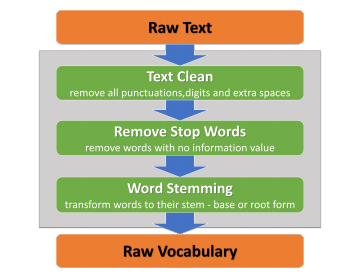
\includegraphics[width=300px, height = 250px]{DataPreprocessFlow.png}
\caption{Data Cleanup Flow}
\label{cleanup_diag}
\end{figure} 

Since we are dealing with real world text reviews, the data available to us will contain plenty of punctation words as well common English stopwords. We followed a standard process for text mining to further cleanse and process the review dataset. In this, we first converted all the reviews to \textbf{lowercase}. We then removed \textbf{numbers} \& \textbf{punctuations}. After this, we \textbf{tokenized} the text using the NLTK library's tokenizer. Post this, we removed the \textbf{stopwords} and we also performed \textbf{stemming} of the words. The cleaned dataset was thus used as an input to all our models trained.
\subsection{Creating Training and Testing Corpus}
We used \textbf{70-30} sampling to create a training and testing corpus from the cleaned text reviews. In order to ensure sufficient representation of all the star label values in our training corpus, we split the \textbf{original corpus on the basis of the star labels}, thus creating 5 corpora, one for each star label. The 70-30 sampling was then carried out on each of the 5 corpora and the training and test files thus created were then combined to create one big training and testing corpus. The number of reviews in training corpus for each star label is given  in Table \ref{corpus_size}.
\begin{table}[!htb]
 \centering
 \caption{Star rating distribution in the training corpora}
 \label{corpus_size}
 \begin{tabular}{l l l} 
    \noalign{\smallskip}\hline\noalign{\smallskip}
    Dataset & Count \\
    \noalign{\smallskip}\hline\noalign{\smallskip}
    Rating 1 &58739\\
    Rating 2 &47154\\
    Rating 3 &72107\\
    Rating 4 &174334\\
    Rating 5 &284902\\
    \noalign{\smallskip}\hline
  \end{tabular} 
\end{table}  
\subsection{LDA Model Development}
The LDA\cite{lda} model is present in \textbf{gensim package} in python. The inbuilt library method was not so straightforward and required a \textbf{vectorized bag of words} corpus as an input. It also required a dictionary developed from the available training corpora. The parameters that could be tweaked while developing the model were the corpora size and the total number of topics we want to extract. We chose the \textbf{total topics as 15}. In a normal vectorized corpus, the dimensionality would have been the entire size of the disctionary, which is very huge. Selecting the total topics essentially will reduce the dimensionality of our training corpora to merely 15 selected topics. The topic probability distribution dataset was used as a feature to create new training corpora which was used to train off the shelf classifiers such as \textit{MultinomialNaiveBayes, LogisticRegression, RandomForestClassifier, AdaBoostClassifier}. The performance of the models is discussed in a separate section on Model Evaluation.

\subsection{Contributions from team members}
All team members had equal contributions to this assignment. (33\% each). The key contributions are as follows : 
\begin{enumerate}
   \item Karan Grover.
   \begin{itemize}
     \item Performed the conversion of json to csv.
     \item Suggested the merger of business and reviews file into one.
     \item Performed the cleaning and pre-processing of the dataset.
   \end{itemize}
   \item Pragya Arora
   \begin{itemize}
   \item Performed the exploratory analysis of the dataset, and suggested using a limit size range of reviews.
   \item Suggested and worked on Bi-Grams, Tri Grams \& Bag of Words approach.
   \item Jointly contributed with Piyush in TF-IDF Vectorized model.
   \end{itemize}
   \item Piyush Ghai
   \begin{itemize}
   \item Suggested to keep the representation of all star labels same in the training and testing split.
   \item Suggested and worked on LDA \& LDA + Sentiment Analysis approaches for classification.
   \end{itemize}
\end{enumerate}

\section{Tools and Technology Stacks}
For this assignment, we've used a variety of tools. The coding for this assignment was done using Python. The following is an exhaustive list of modules/tools used : 
\begin{itemize}
   \item Python 2.7
   \item Pandas (For manipulating the dataframes)
   \item nltk (For corpus, dictionary, stopwords, stemming etc)
   \item NumPy (For classification model results)
   \item seaborn (For graphs)
   \item cPickle (For saving pickle files and using them later in models)
   \item iPython (The interactive python shell, which was used for development)
   \item sci-kit learn (For various classification algorithms)
   \item Gensim (For LDA model)
   \end{itemize}


\newpage
\begin{thebibliography}{}
 \bibitem{yelp}
 Yelp is an American multinational corporation headquartered in San Francisco, California. It develops, hosts and markets Yelp.com and the Yelp mobile app, which publish crowd-sourced reviews about local businesses, as well as the online reservation service Yelp Reservations and online food-delivery service Eat24. \url{https://en.wikipedia.org/wiki/Yelp}. 
 
 \bibitem{yelp_dataset_challenge}
The Yelp Dataset Challenge provides the academic community with a real-world dataset over which to apply their research. More about yelp dataset can be found on :  \url{https://www.yelp.com/dataset_challenge}. 
 
 \bibitem{nltk}
NLTK is a leading platform for building Python programs to work with human language data. It provides easy-to-use interfaces to over 50 corpora and lexical resources such as WordNet, along with a suite of text processing libraries for classification, tokenization, stemming, tagging, parsing, and semantic reasoning, wrappers for industrial-strength NLP libraries. \url{http://www.nltk.org/}. 
 
 \bibitem{lda}
In natural language processing, latent Dirichlet allocation (LDA) is a generative statistical model that allows sets of observations to be explained by unobserved groups that explain why some parts of the data are similar. For example, if observations are words collected into documents, it posits that each document is a mixture of a small number of topics and that each word's creation is attributable to one of the document's topics \url{https://en.wikipedia.org/wiki/Latent_Dirichlet_allocation}. 
  
\end{thebibliography}
\end{document}